\documentclass[12pt]{article}

\usepackage{sbc-template}
\usepackage{graphicx,url}
\usepackage[utf8]{inputenc}
\usepackage[brazil]{babel}
%\usepackage[latin1]{inputenc}  

     
\sloppy

\title{Trabalho Prático de Teoria dos Grafos e Computabilidade\\Processamento e Geração de Grafos}


\author{Rafael M. B. Baptista\inst{1}, Gabriel Felipe S. de Sousa\inst{1}, João Lucas G. Teles\inst{1},
\\Rodrigo A. Rocha\inst{1}, Eron Arthur da Silva\inst{1} }


\address{Instituto de Ciências Exatas e Informática -- Pontifícia Universidade\\Católica de Minas Gerais (PUCMG) }


\begin{document} 

\maketitle

\begin{abstract}
This work presents a computational tool for modeling and analyzing collaboration
networks in open-source GitHub repositories using graph theory concepts. Users
are represented as vertices, while interactions extracted from issues, pull
requests, comments, reviews, approvals, closures, and merges are represented as
directed weighted edges. The tool implements graph structures based on adjacency
lists and adjacency matrices, performs data extraction and processing, computes
centrality, cohesion, structure, and community metrics, and provides visual
interfaces for graph and metric inspection. Two repositories were selected for
analysis: Hyprland, due to its large number of interactions and active
collaboration network, and h3, due to its smaller interaction volume, which
facilitates clearer graph visualization and comparative analysis.
\end{abstract}
     
\begin{resumo}
Este trabalho apresenta uma ferramenta computacional para modelar e analisar
redes de colaboração em repositórios GitHub de código aberto por meio de grafos.
Os usuários são representados como vértices, enquanto interações extraídas de
issues, pull requests, comentários, revisões, aprovações, fechamentos e merges
são representadas como arestas direcionadas e ponderadas. A solução implementa
estruturas de grafos por lista e matriz de adjacência, realiza coleta e
processamento dos dados, calcula métricas de centralidade, estrutura, coesão e
comunidade, e disponibiliza interfaces para visualização dos grafos e resultados.
Foram escolhidos os repositórios Hyprland, por apresentar grande volume de
interações e uma rede colaborativa mais densa, e h3, por possuir quantidade
reduzida de interações, facilitando a visualização e a comparação dos grafos.
\end{resumo}


\section{Introdução}

Projetos de código aberto hospedados no GitHub concentram diferentes formas de
colaboração entre desenvolvedores, como discussões em issues, revisões de pull
requests, aprovações, fechamentos e merges. Essas interações formam uma rede de
relacionamentos que pode ser modelada por grafos, permitindo identificar
colaboradores centrais, grupos de atuação e padrões de coesão dentro da
comunidade do projeto. A análise de redes complexas é amplamente utilizada para
compreender estruturas de relacionamento, centralidade, agrupamentos e fluxos de
informação em sistemas sociais e técnicos~\cite{newman2010networks}.

Este trabalho desenvolve uma ferramenta computacional para extrair, processar,
modelar e analisar interações entre usuários de repositórios GitHub, usando
conceitos de teoria dos grafos. Cada usuário é representado como um vértice, e
cada interação entre usuários é representada como uma aresta direcionada e
ponderada. A ferramenta implementa duas estruturas de representação de grafos,
lista de adjacência e matriz de adjacência, além de módulos de coleta,
processamento, cálculo de métricas, exportação e visualização.

Foram escolhidos dois repositórios para análise: \textit{Hyprland}
(\texttt{hyprwm/Hyprland}) e \textit{h3} (\texttt{h3js/h3}). O Hyprland foi
selecionado por apresentar um grande volume de interações e uma comunidade ativa,
permitindo observar uma rede colaborativa mais densa. O h3 foi escolhido por
possuir uma quantidade menor de interações, facilitando a visualização dos
grafos e a comparação dos resultados obtidos.

\section{Modelagem do Problema}

A modelagem proposta considera que cada usuário participante das interações do
repositório é um vértice do grafo. As interações entre usuários são convertidas
em arestas direcionadas, indicando a origem e o destino da relação. Por exemplo,
quando um usuário comenta em uma issue aberta por outro usuário, cria-se uma
aresta do autor do comentário para o autor da issue. Quando um usuário fecha uma
issue criada por outro, cria-se uma aresta representando essa ação.

Foram construídos três grafos específicos e um grafo integrado:

\begin{itemize}
    \item \textbf{Grafo 1 -- Comentários}: representa comentários em issues e
    pull requests.
    \item \textbf{Grafo 2 -- Fechamentos}: representa fechamentos de issues por
    usuários diferentes dos autores.
    \item \textbf{Grafo 3 -- Reviews e merges}: representa revisões, aprovações
    e merges em pull requests.
    \item \textbf{Grafo 4 -- Integrado}: combina todas as interações anteriores
    em um único grafo ponderado.
\end{itemize}

As arestas possuem pesos para representar a intensidade das interações. Assim,
interações mais relevantes no processo colaborativo, como revisões e merges,
podem ter maior influência nas métricas do grafo do que interações mais simples,
como comentários.

\section{Repositórios Analisados}

Para a realização deste trabalho, foram selecionados dois repositórios públicos
do GitHub: \texttt{hyprwm/Hyprland} e \texttt{h3js/h3}. A escolha considerou
tanto a relevância dos projetos quanto a diferença no volume de interações
entre suas comunidades, permitindo avaliar a ferramenta em cenários distintos.

O Hyprland é um compositor Wayland dinâmico para ambientes Linux, voltado à
construção de uma experiência de desktop moderna, com janelas em mosaico,
animações e alto grau de personalização~\cite{hyprlandDocs}. Por ser um projeto
de infraestrutura gráfica utilizado por muitos usuários e colaboradores, seu
repositório apresenta um volume elevado de issues, pull requests, comentários,
revisões e merges. Essa característica torna o Hyprland um estudo de caso
adequado para observar redes colaborativas mais densas, identificar usuários
centrais, comunidades internas e possíveis pontes entre grupos de
desenvolvimento.

O h3 é uma biblioteca geoespacial criada originalmente pela Uber para indexação
hierárquica da superfície terrestre por meio de células hexagonais
\cite{h3Docs}. O repositório \texttt{h3js/h3} corresponde à implementação em
JavaScript dessa tecnologia, sendo usado em aplicações de mapas, análise
espacial, visualização de dados geográficos e processamento de informações
baseadas em localização. Em comparação com o Hyprland, o h3 possui uma
quantidade menor de interações no conjunto analisado, o que facilita a
visualização dos grafos gerados e a interpretação manual das relações entre
usuários.

Assim, os dois repositórios foram escolhidos de forma complementar. O Hyprland
permite testar a solução em um cenário com maior quantidade de interações e
maior complexidade estrutural, enquanto o h3 oferece um cenário mais reduzido,
adequado para validação visual da ferramenta e comparação dos resultados.

\section{Estruturas de Dados e Implementação}

A implementação foi organizada em módulos responsáveis por etapas específicas
do fluxo de execução. O módulo \texttt{ExtracaoDados} realiza a comunicação com
a API GraphQL do GitHub, coleta issues e pull requests e salva os dados brutos
em arquivos JSON. Em seguida, o módulo \texttt{InteractionParser} transforma os
dados brutos em interações padronizadas, separadas em arquivos processados.

Um exemplo de estrutura processada utilizada para representar uma aresta é
apresentado a seguir:

\begin{verbatim}
{
  "de": "usuario_origem",
  "para": "usuario_destino",
  "peso": 2
}
\end{verbatim}

Após o processamento, o módulo \texttt{MapeamentoVertices} cria um mapeamento
entre nomes de usuários e identificadores numéricos. Esse mapeamento é usado na
construção dos grafos:

\begin{verbatim}
{
  "global": {
    "mapeamento": {
      "usuario_a": 0,
      "usuario_b": 1,
      "usuario_c": 2
    }
  }
}
\end{verbatim}

A construção dos grafos é feita pela classe \texttt{Construcao}, que instancia
duas representações: \texttt{AdjacencyListGraph} e
\texttt{AdjacencyMatrixGraph}. Ambas herdam de \texttt{AbstractGraph}, uma classe
abstrata que define a API comum exigida pelo trabalho, incluindo métodos para
adição e remoção de arestas, consulta de pesos, graus de entrada e saída,
verificação de conectividade e exportação para formatos compatíveis com Gephi.

\begin{figure}[ht]
\centering
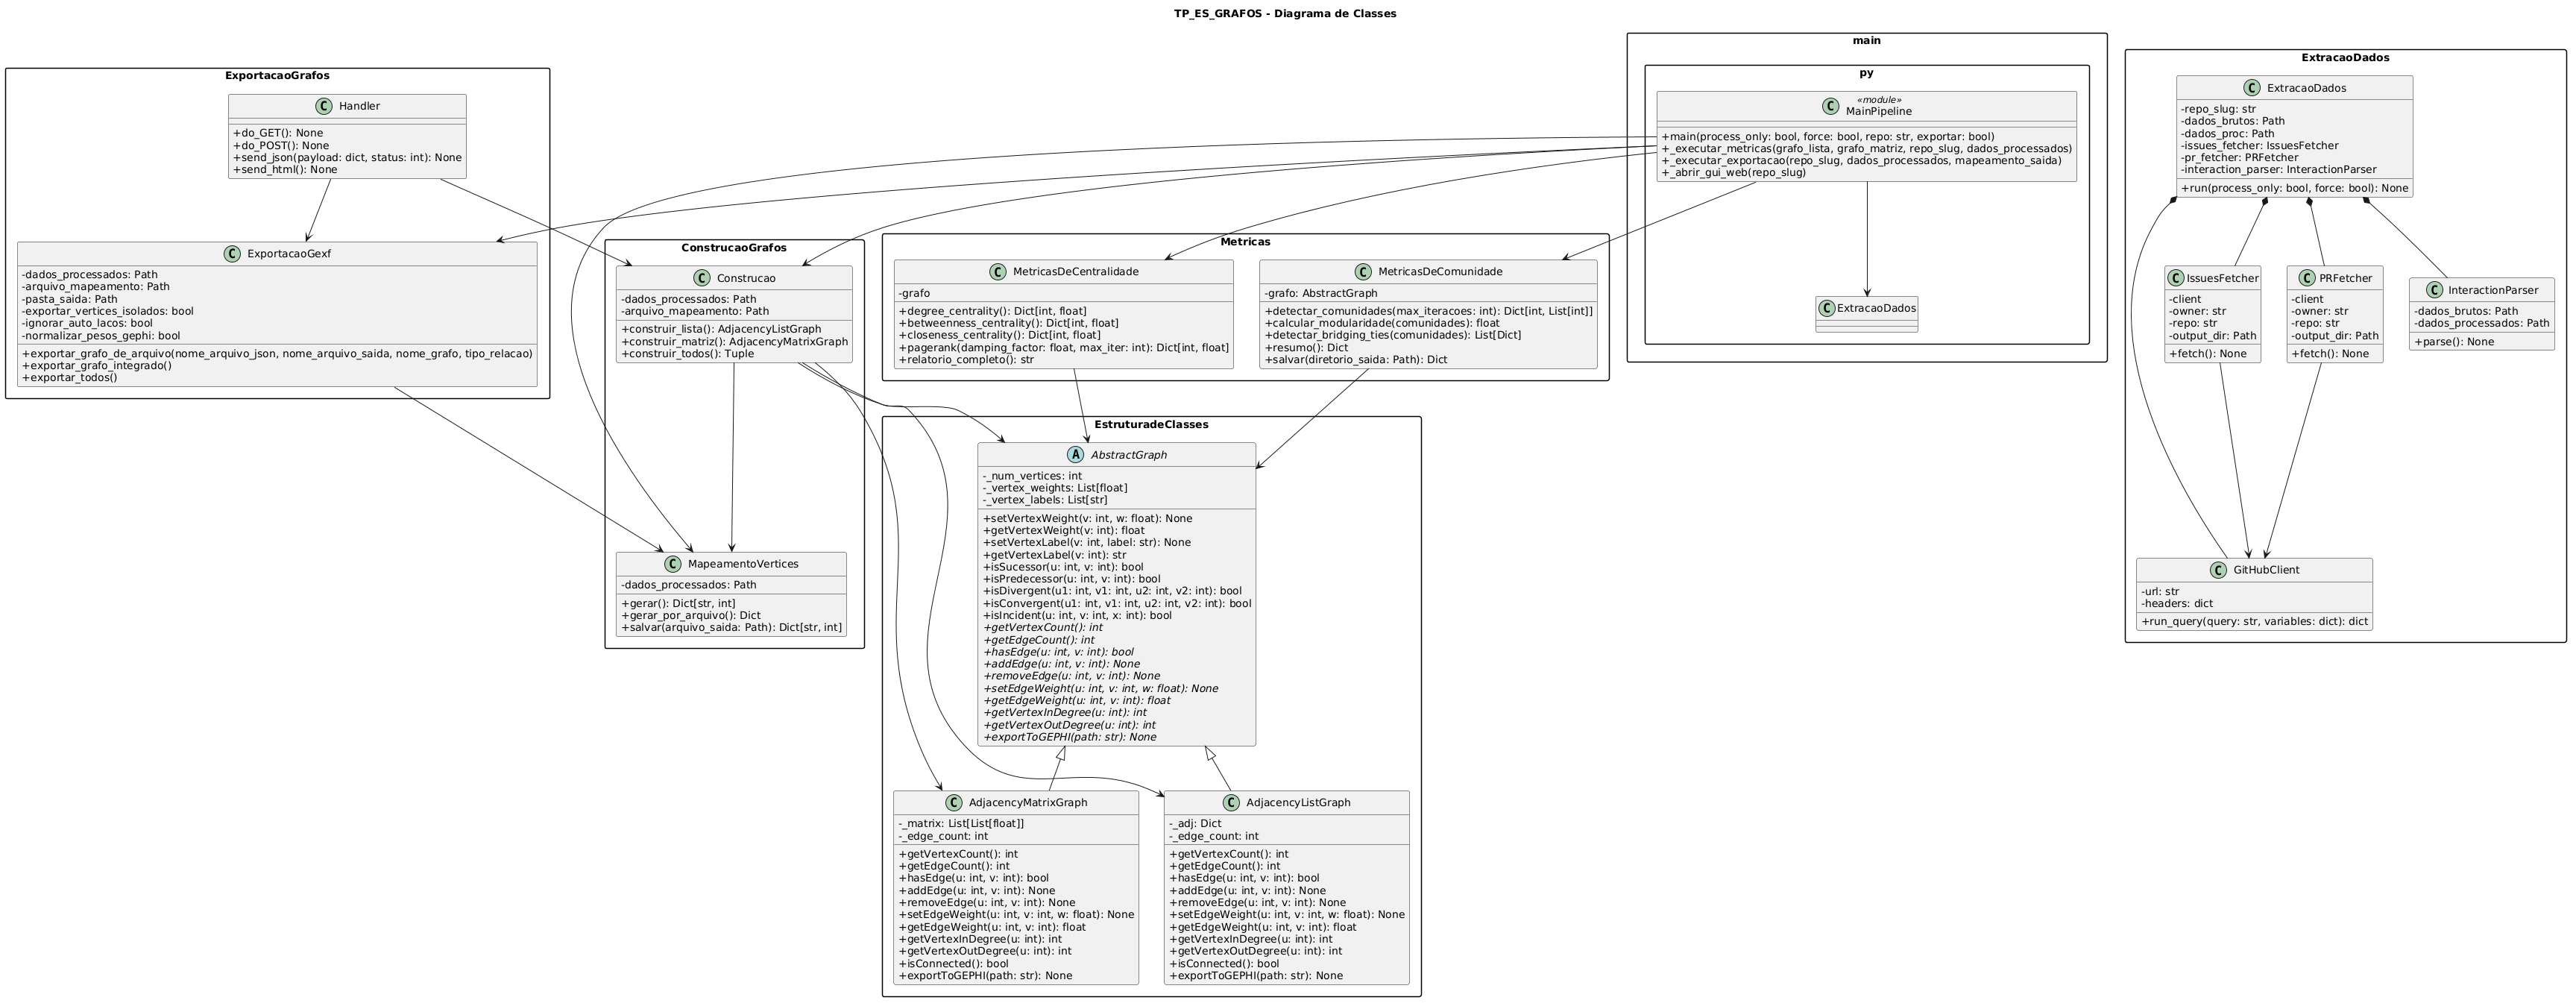
\includegraphics[width=0.95\textwidth]{figuras/diagrama_classes.png}
\caption{Diagrama de classes da ferramenta desenvolvida.}
\label{fig:diagrama-classes}
\end{figure}

\section{Métricas Calculadas}

A ferramenta calcula métricas de centralidade, estrutura, coesão e comunidade.
As métricas de centralidade permitem identificar usuários com maior influência
ou participação na rede. A centralidade de grau indica a quantidade de conexões
diretas de um vértice, enquanto a centralidade de intermediação permite observar
vértices que atuam como pontes entre diferentes regiões do grafo
\cite{freeman1978centrality}. Também são calculadas a centralidade de
proximidade e o PageRank, métrica originalmente proposta para ranqueamento de
páginas na Web, mas aplicável a grafos direcionados em geral
\cite{page1999pagerank}.

As métricas de estrutura e coesão incluem densidade, coeficiente de
aglomeração e assortatividade por grau. A densidade indica o quanto a rede se
aproxima de um grafo completamente conectado. O coeficiente de aglomeração mede
a tendência dos usuários formarem grupos locais, enquanto a assortatividade
indica se vértices com graus semelhantes tendem a se conectar entre si
\cite{newman2002assortative}.

Por fim, as métricas de comunidade permitem identificar grupos de usuários com
maior frequência de interação entre si. A detecção de comunidades é uma
abordagem comum na análise de redes sociais e biológicas, pois evidencia
subestruturas internas em redes complexas~\cite{girvan2002community}. Também
são analisados \textit{bridging ties}, isto é, usuários que conectam
comunidades diferentes e atuam como pontes na rede colaborativa.

\section{Interface e Visualização}

Além da execução por linha de comando, foi desenvolvida uma interface web local
para facilitar a visualização dos resultados. A interface permite escolher o
repositório analisado, executar o pipeline de processamento, visualizar métricas
resumidas, consultar rankings de centralidade, observar comunidades detectadas
e inspecionar uma amostra visual do grafo.

Os grafos também podem ser exportados no formato GEXF, compatível com o Gephi,
ferramenta amplamente utilizada para exploração e visualização de redes
\cite{bastian2009gephi}. Essa exportação permite que os resultados produzidos
pela ferramenta sejam analisados em softwares externos especializados.

\begin{figure}[ht]
\centering
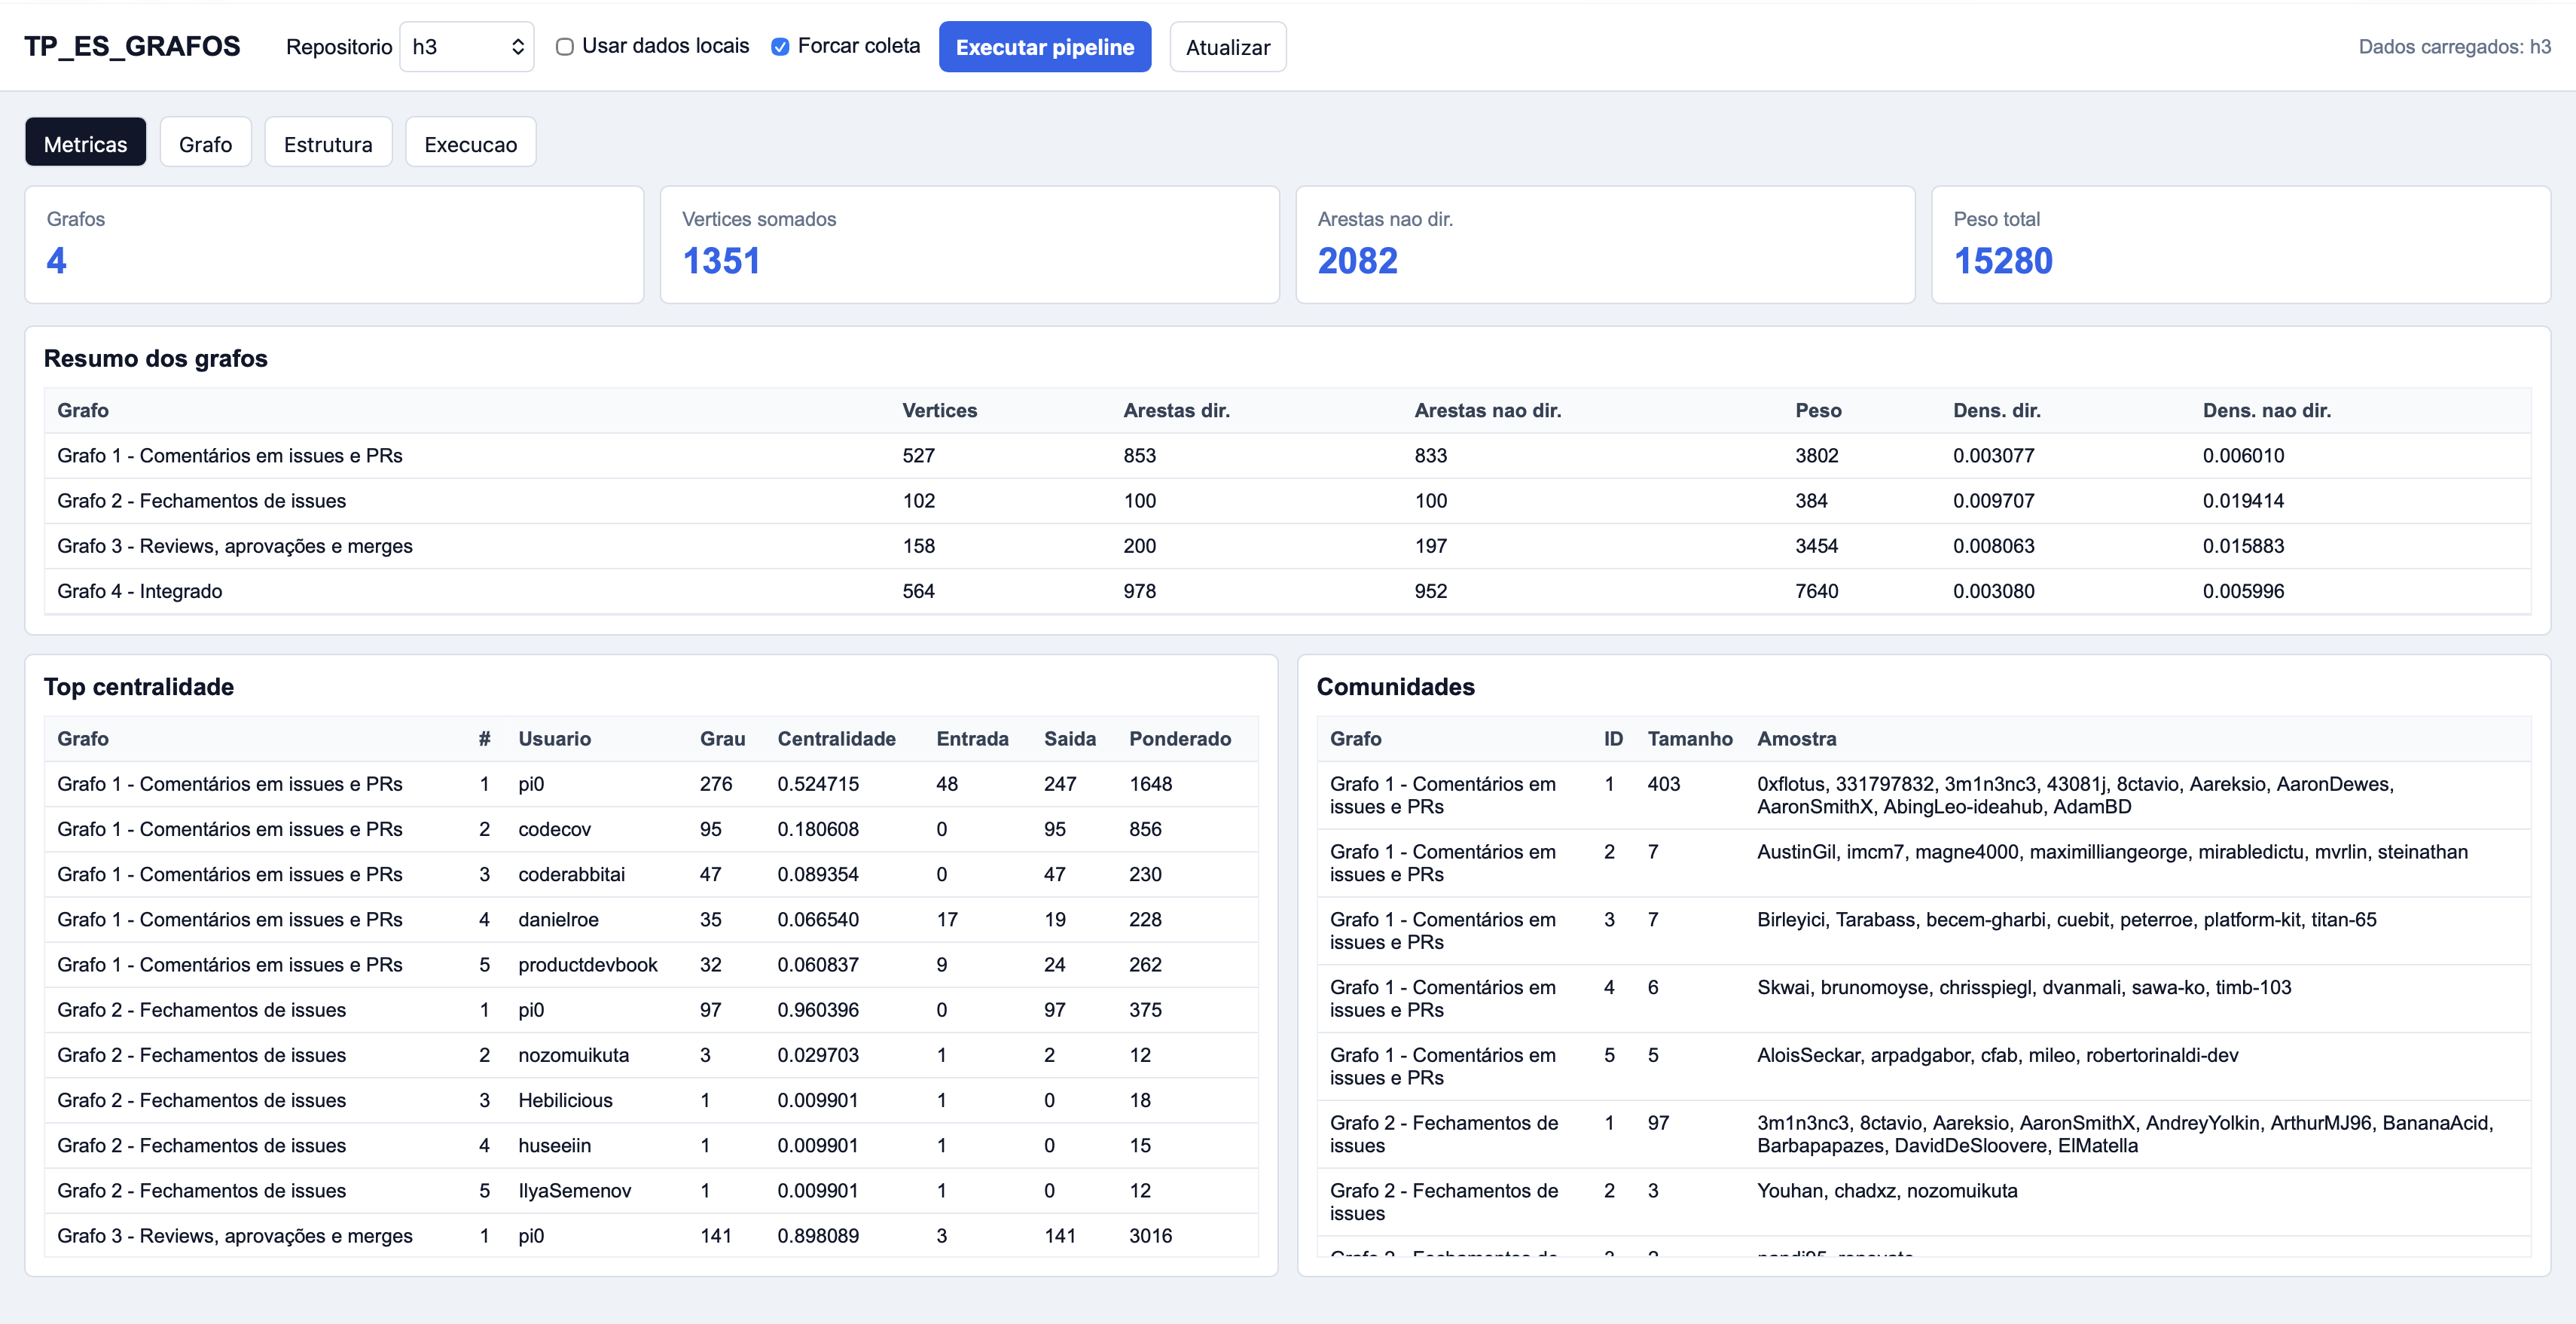
\includegraphics[width=0.95\textwidth]{figuras/tela_metricas.png}
\caption{Tela da interface web com resumo das métricas dos grafos.}
\label{fig:tela-metricas}
\end{figure}

A Figura~\ref{fig:tela-grafo} apresenta a visualização gráfica de uma amostra
do grafo integrado. Essa visualização é especialmente útil no repositório h3,
pois a menor quantidade de interações facilita a inspeção visual das relações
entre usuários.

\begin{figure}[ht]
\centering
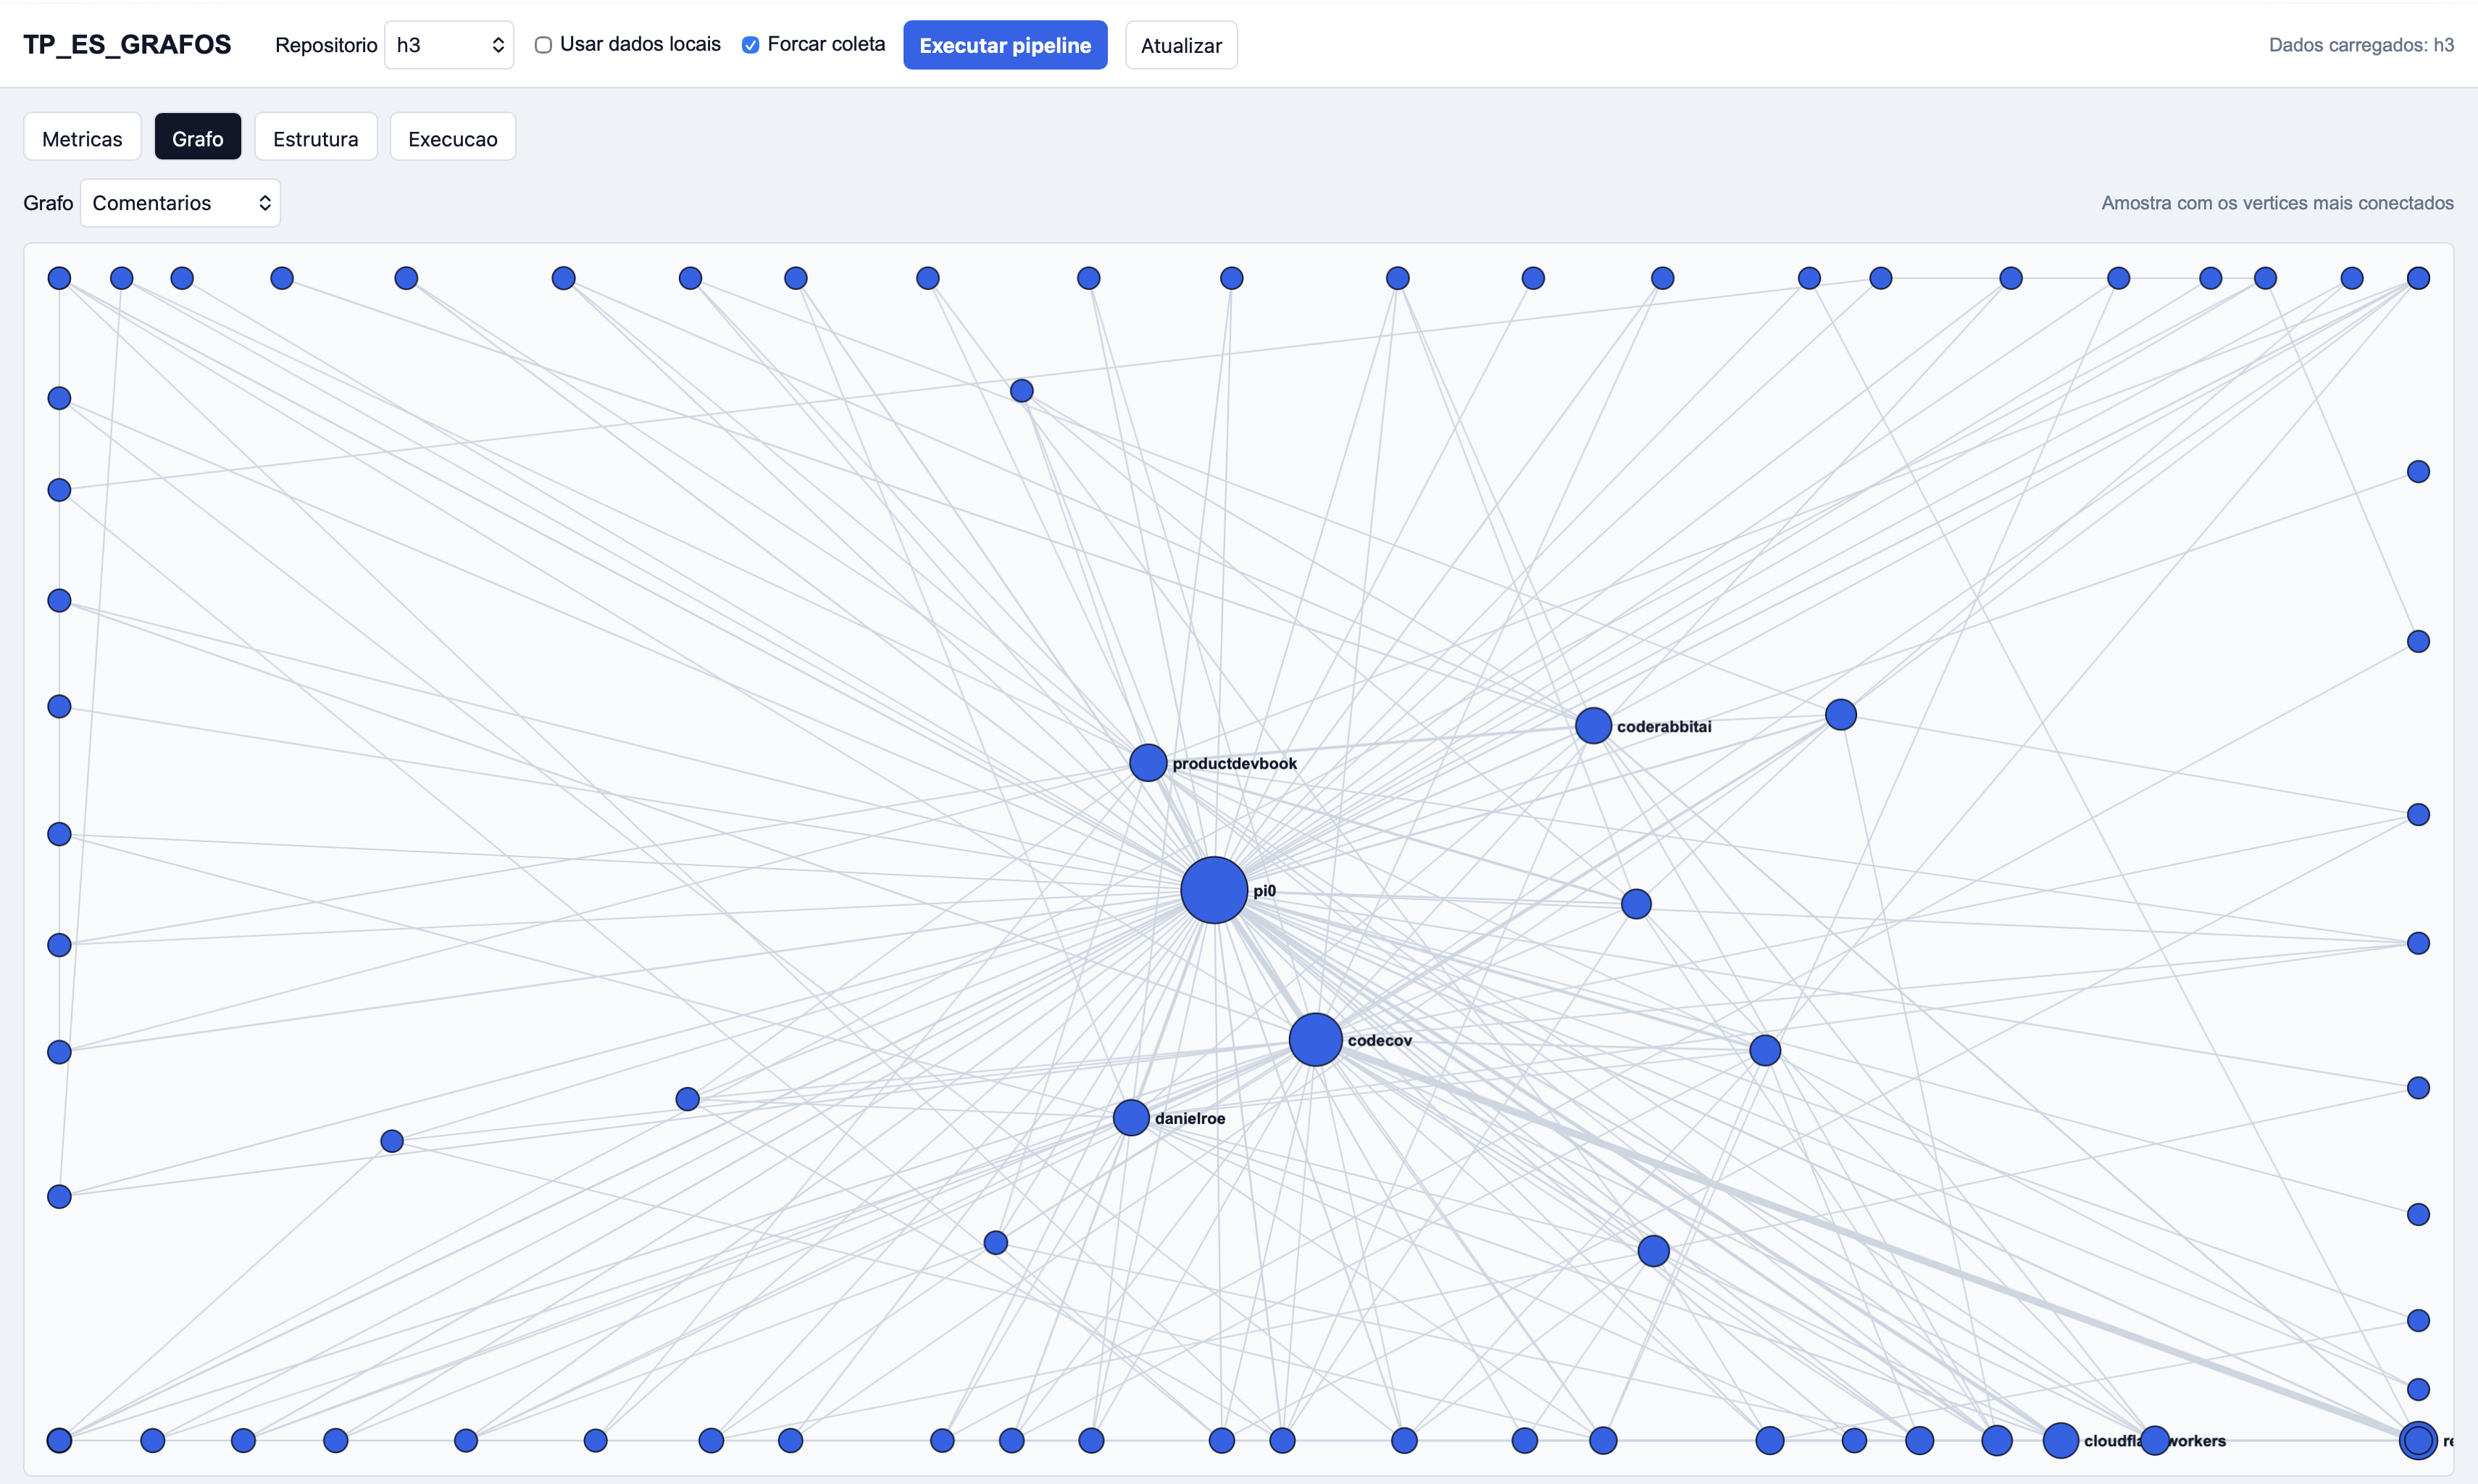
\includegraphics[width=0.95\textwidth]{figuras/tela_grafo.png}
\caption{Visualização do grafo integrado na interface web.}
\label{fig:tela-grafo}
\end{figure}

A Figura~\ref{fig:tela-execucao} mostra a aba de execução, utilizada para
acompanhar os logs do pipeline quando a coleta ou o processamento são acionados
pela interface.

\begin{figure}[ht]
\centering
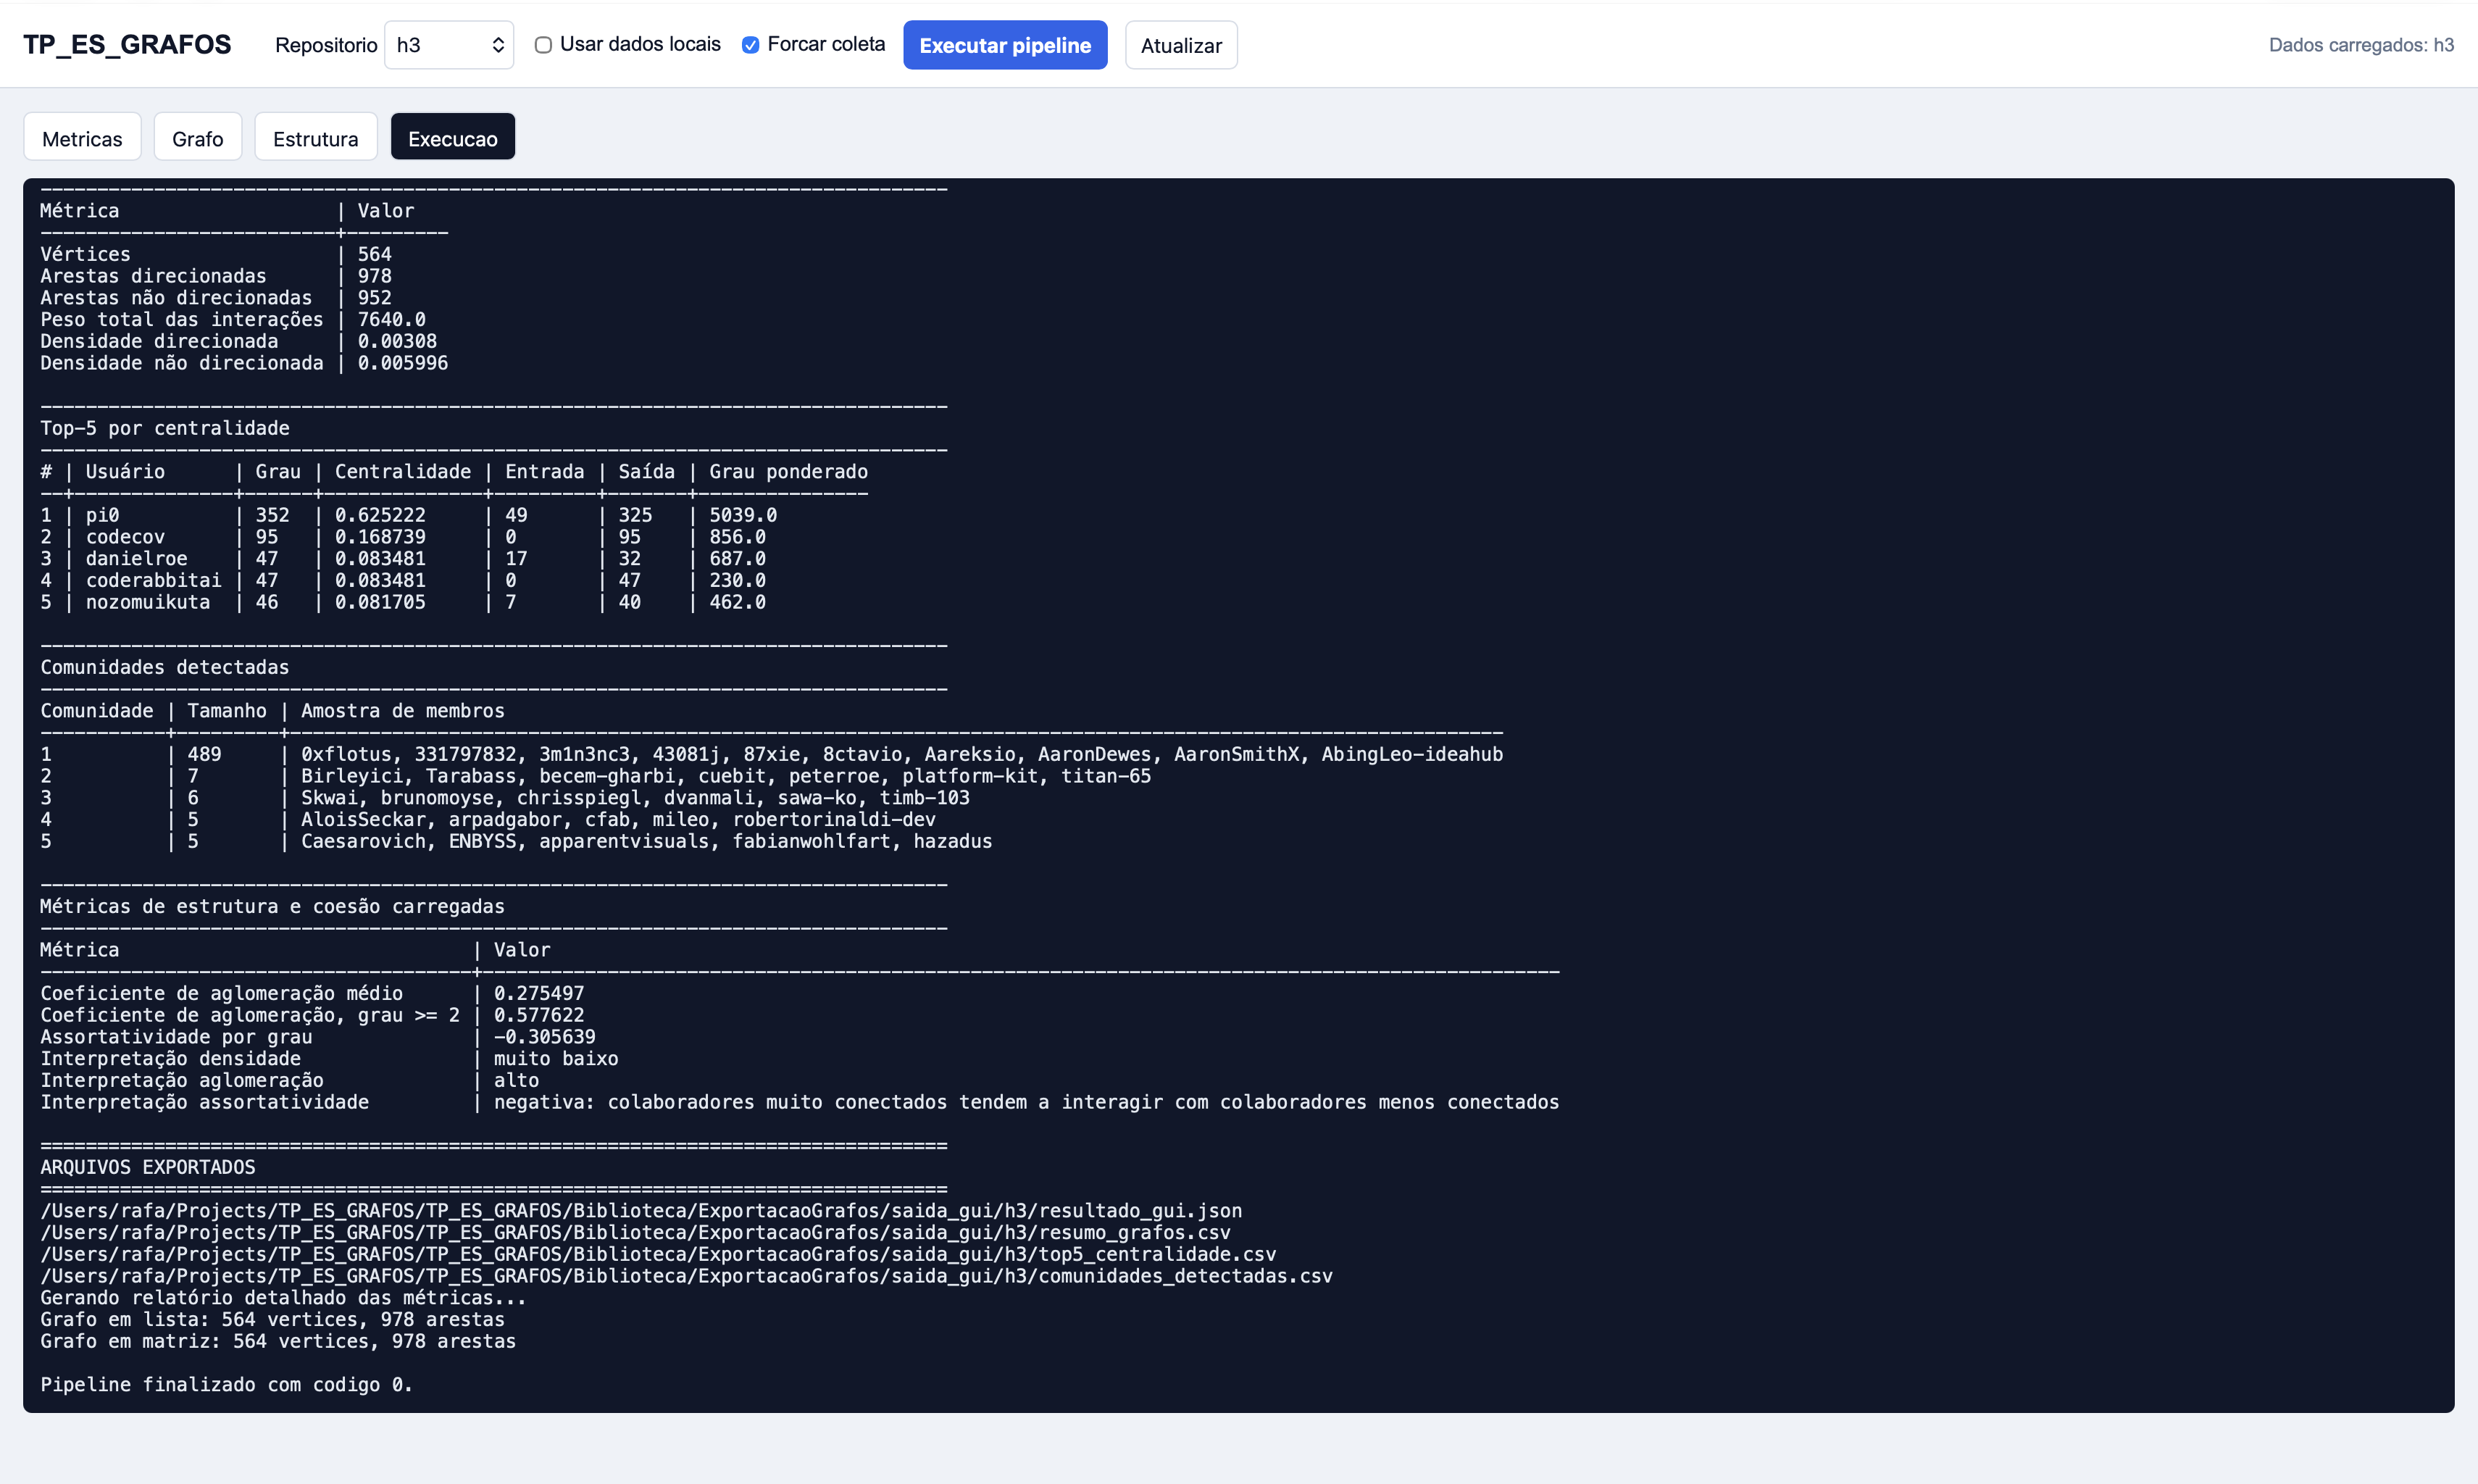
\includegraphics[width=0.95\textwidth]{figuras/tela_execucao.png}
\caption{Aba de execução exibindo logs do pipeline.}
\label{fig:tela-execucao}
\end{figure}

\section{Execução da Ferramenta}

A ferramenta pode ser executada diretamente pelo arquivo \texttt{main.py}, que
coordena as etapas de extração, processamento, construção dos grafos, cálculo
das métricas e exportação dos resultados. A execução principal recebe como
parâmetro o repositório analisado, permitindo selecionar entre \texttt{h3} e
\texttt{hyprland}. Também é possível executar apenas o processamento dos dados
locais, sem realizar nova coleta na API do GitHub, por meio da opção
\texttt{--process-only}.

\begin{verbatim}
python Biblioteca/main.py --repo h3 --process-only
\end{verbatim}

Após a execução, os resultados são organizados em arquivos JSON e CSV,
utilizados tanto pela interface web quanto pelas exportações para visualização
externa. A interface web local também permite acionar o pipeline, atualizar os
dados exibidos e consultar os logs da execução. Dessa forma, a aplicação
separada exigida no enunciado é usada para consumir a API implementada e
demonstrar as operações disponíveis.

\section{Testes e Validação}

Foram desenvolvidos testes unitários para validar as principais partes da
solução. Na estrutura de grafos, os testes verificam o comportamento da classe
abstrata \texttt{AbstractGraph} e das implementações concretas
\texttt{AdjacencyListGraph} e \texttt{AdjacencyMatrixGraph}. Esses testes
cobrem operações como criação de grafos, adição e remoção de arestas,
verificação de existência de arestas, consulta de graus, pesos de vértices e
arestas, conectividade, grafo vazio, grafo completo e exportação.

Também foram implementados testes para a etapa de extração e processamento dos
dados. Esses testes validam o cliente GitHub, os coletores de issues e pull
requests, e o parser responsável por transformar os dados brutos em interações
processadas. Além disso, há testes para a construção dos grafos a partir dos
arquivos JSON processados, verificando se os pesos são acumulados corretamente,
se os rótulos dos vértices são atribuídos e se as representações por matriz e
lista produzem resultados equivalentes.

Essa validação contribui para garantir que a ferramenta respeita as restrições
do enunciado, como não permitir laços, evitar múltiplas arestas, lançar
exceções para operações inconsistentes e manter a compatibilidade entre as duas
representações de grafos.

\section{Resultados Obtidos e Comparação dos Repositórios}

A análise dos dois repositórios permite observar comportamentos distintos. No
Hyprland, a maior quantidade de interações gera uma rede mais complexa, com
maior número de vértices e arestas, favorecendo a análise de centralidade,
comunidades e pontes entre grupos. Esse repositório é adequado para observar
fenômenos típicos de redes colaborativas maiores, como concentração de
interações em usuários centrais e formação de subcomunidades.

No h3, a quantidade reduzida de interações permite uma visualização mais clara
dos grafos gerados. Esse repositório foi utilizado como contraponto ao
Hyprland, facilitando a validação visual da ferramenta e a compreensão das
estruturas produzidas. Assim, a escolha dos dois repositórios contribui para
avaliar a solução tanto em um cenário com maior volume de dados quanto em um
cenário mais simples e visualmente interpretável.

No conjunto processado pela ferramenta, o grafo de comentários possui 527
vértices, 853 arestas direcionadas e peso total de 3802 interações. O grafo de
fechamentos possui 102 vértices e 100 arestas direcionadas, enquanto o grafo de
reviews, aprovações e merges possui 158 vértices e 200 arestas direcionadas. O
grafo integrado consolida as interações e apresenta 564 vértices, 978 arestas
direcionadas, 952 arestas não direcionadas e peso total de 7640 interações.
Esses resultados evidenciam que a ferramenta consegue consolidar diferentes
tipos de colaboração em uma única estrutura analisável, mantendo também grafos
separados para inspeções específicas.

\section{Divisão de Responsabilidades}

A divisão de responsabilidades entre os integrantes do grupo foi organizada de
forma a cobrir as principais etapas do desenvolvimento da ferramenta, desde a
extração dos dados até a documentação e apresentação dos resultados.

\begin{itemize}
    \item \textbf{Rafael}: documentação e implementação do frontend do projeto.
    \item \textbf{Eron}: desenvolvimento da extração dos dados, produção do
    vídeo, implementação das métricas de centralidade e elaboração dos slides
    da apresentação.
    \item \textbf{João}: desenvolvimento dos testes da parte 2 do trabalho e
    criação da aplicação demo.
    \item \textbf{Gabriel}: preparo das exportações dos dados relevantes para a
    criação da GUI e implementação das métricas de estrutura e coesão.
    \item \textbf{Rodrigo}: desenvolvimento da construção dos grafos a partir
    dos dados extraídos e README principal da aplicação.
\end{itemize}

\section{Conclusão}

Este trabalho apresentou uma ferramenta para análise de colaboração em
repositórios GitHub utilizando grafos direcionados e ponderados. A solução
implementa coleta de dados, processamento de interações, construção de grafos em
lista e matriz de adjacência, cálculo de métricas e visualização por interface
web local.

A escolha dos repositórios Hyprland e h3 permitiu avaliar a ferramenta em dois
cenários complementares: um com grande volume de interações, adequado para
análises mais densas de redes colaborativas, e outro com menor volume de dados,
mais apropriado para inspeção visual. Com isso, a ferramenta demonstra a
aplicabilidade de conceitos de teoria dos grafos na compreensão da dinâmica de
colaboração em projetos de código aberto.

\bibliographystyle{sbc}
\bibliography{sbc-template}

\end{document}
